
\section{Durchführung}
\label{sec:Durchführung}
\subsection{Aufbau}
\begin{figure}
\centering
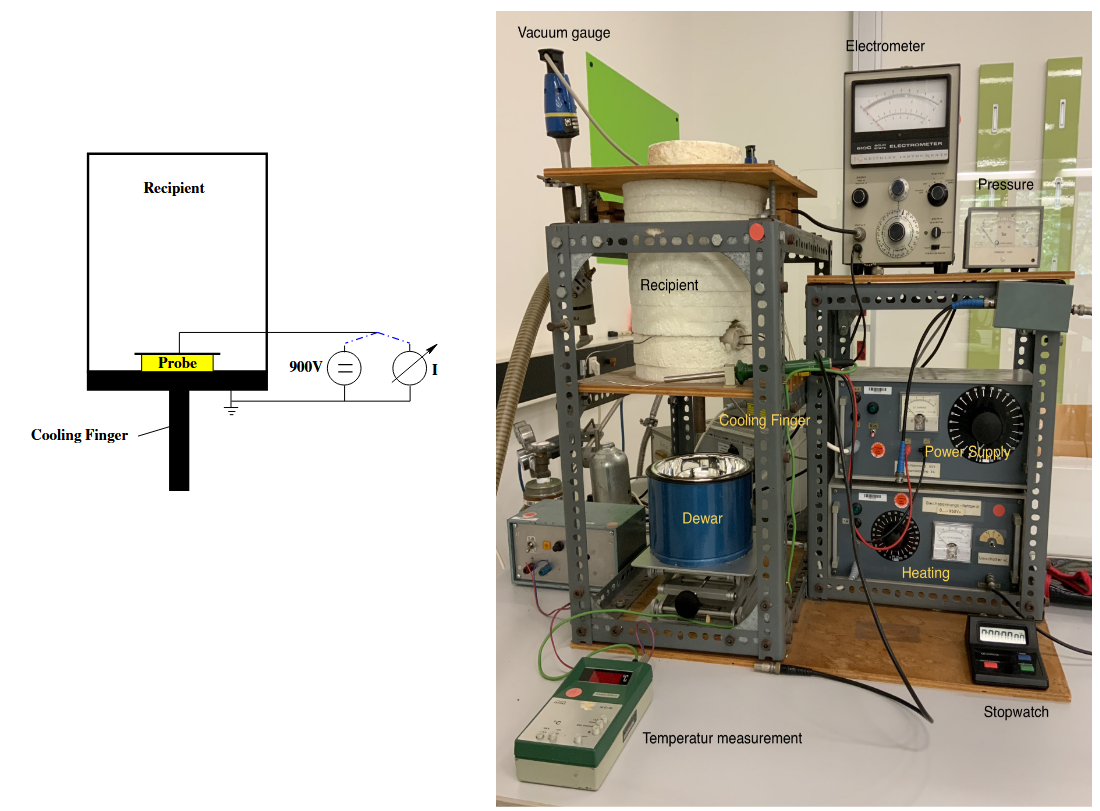
\includegraphics[width=\textwidth,keepaspectratio]{Dipolrelaxation Versuchsanordnung}
\label{fig:Versuchsanordnung}
\caption{Gesamte Versuchsanordnung, die in diesem Versuch verwendet wurde inklusive entsprechender Beschriftung (rechts) und schematische Veranschaulichung  des Rezipienten (links).}
\end{figure}
Der Aufbau, der für diesen Versuch verwendet wird, lässt sich Abbildung $\ref{fig:Versuchsanordnung}$ entnehmen. Die Probe befindet sich im Rezipienten, in dem durch eine Pumpe ein Vakuum von $\SI{10}{\milli\bar}$ bis $\SI{10}{\milli\bar}$ erzeugt wird, um Störeffekte durch Luftfeuchtigkeit zu vermeiden.
Auf der Probe ist eine Metallplatte, welche mit dem Rezipientenboden als Erdung einen Plattenkondensator bildet, um die Probe polarisieren zu können. Die Probe ist außerdem zu Heizzwecken mit einer Heizspule umwickelt. Unten am Rezipienten befindet sich ein Kühlungsfinger der durch Flüssigstickstoff in einem Dewargefäß kann zur Kühlung der Probe verwendet werden kann. Die Temparatur und der Depolarisationstrom können an der können an den entsprechenden Messgeräten abgelesen werden.
\subsection{Messreihen}
Zur Durchführung der Messung muss die Probe zunächst aufgeheizt werden. Bei aufgeheizter Probe wird dann der Plattenkondensator eingeschaltet, um die Probe zu polarisieren. Dabei muss die Zeit, in der das E-Feld wirkt muss dabei groß gegenüber der Relaxationsdauer sein. Sobald die Probe ausreichend polarisiert wurde wird der Flüssigstickstoff verwendet, um die Probe langsam auf eine Temparatur von ca. $\SI{-50}{\celsius}$ bis $\SI{-60}{\celsius}$ zu kühlen. Anschließend wird der Kondensator abgeschaltet und für ca. $\SI{5}{\min}$ kurzgeschlossen. Nachdem der Kondensator vollständig entladen ist wird das Picoamperemeter angeschlossen und die Probe wird wieder aufgeheizt bis zu einer Temparatur von circa $\SI{50}{\celsius}$. Dabei werden jeweils einmal pro Minute Depolarisationsstrom und Temparatur gemessen. Um eine möglichst Konstante heizrate zu erreichen muss während des Heizprozesses die Heizspannung immer wieder angepasst werden. Diese Prozedur wird für zwei unterschiedliche konstante Heizraten wiederholt.